\chapter{Úvod}
Webové portály jsou v~současné době nedílnou součástí internetu. Shromažďují informace z~vícero různých zdrojů a ty nejrelevantnější prezentují uživatelům shromážděné na jednom místě~\cite{bib:portal-liferay}. \blindtext

Cílem práce je rozšíření stávajícího portálu, zaměřeného na výsledky evropských projektů. Od vytvoření tohoto portálu již uplynulo několik let, a proto bylo třeba jej upravit pro použití novějších verzí knihoven. Při této činnosti bylo kompletně přepracováno uživatelské rozhraní portálu. Dále byl obsah tohoto portálu rozšířen o témata nově vypsaných výzev. % TODO doporucovani podobnych

Pro toto téma jsem se rozhodl, protože mám k~webovým technologiím blízko již od dětství a chci v~tomto směru nadále rozvíjet své znalosti.

Tato práce vychází z~bakalářské práce \emph{Automaticky aktualizovaný webový portál} Petra Staňka~\cite{bib:stanek}.
Webový portál byl od základu implementován znovu s~použitím modernějších technologií. Extrakce dat zůstala zachována, pouze byla rozšířena o~extrakci témat výzev k~předkládání návrhů.

V~druhé kapitole práce, nazvané \uv{Rozbor řešené problematiky}, nejprve stručně shrnu základní principy vývoje webových stránek, poté přiblížím několik technologií, které jsem při tvorbě této bakalářské práce využil.
Ve třetí kapitole s~názvem \uv{Návrh a implementace systému} se již zaměřím na konkrétní řešení této práce, uvedu několik obrázků z~výsledného portálu, jež je výsledkem této práce, a popíšu několik zajímavých částí samotného kódu.
Ve čtvrté kapitole pojmenované \uv{Experimenty a vyhodnocení} provedu s výsledným portálem několik experimentů, následně vyhodnotím jejich výstupy a vyvodím z nich možná rozšíření portálu.
V~samém závěru práce pak stručně zhodnotím výsledky této práce.




\chapter{Rozbor řešené problematiky}
Tato kapitola v~úvodu přibližuje základní koncepci vývoje webu a praktiky, které jsou při tomto vývoji často využívány. Následně jsou v~této kapitole popsány jazyky a knihovny, využívané při implementaci této bakalářské práce. V samém závěru kapitoly je přiblížena koncepce podobnostního hledání.



\section{Vývoj webu}
\emph{Tato kapitola čerpá z~\cite{bib:web-development}}.

Z pohledu vývoje nejen webových stránek je zvykem projekt rozlišovat do dvou vrstev. Tou první je klientská část (anglicky \emph{frontend}) a druhou je serverová část (anglicky \emph{backend}).

Klientská část webu je to, co uživatel vidí, když stránku navštíví. Sestavení této části se v~žádném případě neobejde bez značkovacího jazyka HTML (\emph{Hypertext Markup Language}), který udává strukturu a obsah webové stránky. Další nedílnou součástí jsou kaskádové styly neboli CSS (\emph{Cascading Style Sheets}). Ty ovlivňují, jak bude obsah stránky esteticky působit. Další součástí, se kterou se setkáte téměř na každém webu, je skriptovací jazyk JavaScript, který umožňuje webové stránky obohatit o~interaktivitu.
Zpracování této části webu probíhá na straně klienta - tedy internetovému prohlížeči uživatele. Na základě tohoto faktu lze každé stránce na internetu \uv{nahlédnout pod pokličku} a zdrojové kódy klientské části zobrazit. Ve většině případů je možné i~rovnou v~internetovém prohlížeči tyto kódy upravit, což má samozřejmě vliv jen pro současného uživatele a ostatním návštěvníkům webu se tyto změny nijak neprojeví.

Oproti tomu serverová část je od uživatele izolována a zdrojové kódy pro něj nejsou přístupné, pokud je sám autor někde nezveřejní. Jejich interpretace totiž probíhá přímo na serveru a ten poté klientovi odešle již zpracovanou odpověď, obsahující pouze zdrojové kódy klientské části. Výběr technologie implementace serverové části je podstatně rozmanitější, patří mezi ně například Python, PHP, Java, C\#, C++, .NET, Ruby a další. Díky prostředí Node.js\footnote{Node.js: \url{https://nodejs.org/en/}} lze ale využít i~dříve zmiňovaný JavaScript, který pro tento účel nebyl primárně určen. 


\subsection{Architektura MVC}
\emph{Tato kapitola čerpá z~\cite{bib:mvc}}.

Většinu aplikací lze obecně rozdělit na tři hlavní celky - data, rozhraní a logiku. V~anglickém jazyce se tyto celky označují pojmy \emph{model}, \emph{view} a \emph{controller} (zkratka MVC). Historie této architektury sahá až do sedmdesátých let, nicméně i v~dnešní době je stále naprostým standardem vývoje. Schéma zmíněné architektury je znázorněno v~grafu~\ref{img:mvc}.

\begin{figure}[H]
	\centering
	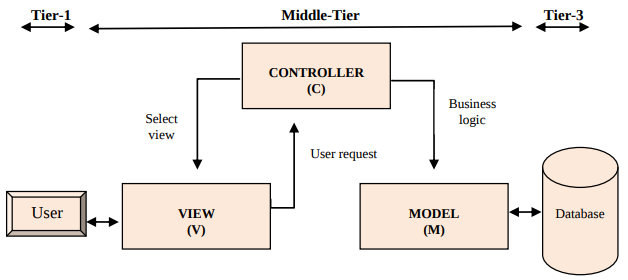
\includegraphics[width=\textwidth]{obrazky-figures/mvc.png}
	\caption{Diagram toku akcí při využití architektury MVC. \emph{Převzato z~\cite{bib:mvc}}}
	\label{img:mvc}
\end{figure}

\begin{itemize}
\item Pojmem pohled (\emph{view}) se označuje uživatelské rozhraní (například stránka zobrazená v~prohlížeči), tato vrstva prezentuje data a je to také jediná vrstva, s~kterou uživatel přímo komunikuje. Akce provedené v~pohledu se předají kontroleru ke zpracovaní.
\item Kontroler (\emph{controller}) se chová jako prostředník mezi daty a rozhraním, zpracovává požadavky uživatele a provede s~modelem potřebné akce. Ve většině případů po provedené akci kontroler znovu obnoví pohled.
\item Model je obvykle objekt obsahující patřičná data z~databáze. Zprostředkovává jak jejich získání, tak i~ukládání. Mimo to může být objekt obohacen i~o~funkce, zpracovávající tyto data (například může převádět Unixový čas do formátu lépe čitelného pro člověka). 
\end{itemize}


Oddělením těchto celků je zajištěna lepší organizovanost zdrojových kódů, a tím je usnadněn rychlejší vývoj. Jednotlivé celky jsou také snadněji znovupoužitelné a práce programátorů na nich může probíhat souběžně. Díky rozdělení je také možné pro jeden model mít pohledů hned několik. Další pohledy mohou přibývat nebo naopak ty stávající mohou být smazány a na databázi aplikace to nebude mít žádný vliv.


\subsection{Responzivita}\label{section:responsive}
\emph{Tato kapitola čerpá z~\cite{bib:responsive}}.

Responzivní design, jak název vypovídá, je design, který je schopný reagovat. Stránka, která má takový design, se přizpůsobuje zařízení, na kterém je právě zobrazena. Díky tomu lze pohodlně prohlížet tu stejnou webovou stránku jak na desktopovém, tak i mobilním zařízení. 

Před několika lety bylo zvykem tvořit webové stránky s~pevnou šířkou obsahu. Tato šířka byla volena tak, aby bylo možné stránku zobrazit jak na starších monitorech s~poměrem stran 4:3, tak i~na modernějších širokoúhlých monitorech. 

Se stále rostoucí oblibou a dostupností chytrých telefonu se ale pro vývojáře a designéry objevila nová výzva. Bylo potřeba webové stránky přizpůsobit i~pro tyto zařízení s~různorodou velikostí obrazovky. Webovou stránku, která nenabízí responzivní design, sice je možné zobrazit i na mobilním zařízením, ale prohlížení takové stránky zpravidla není pro uživatele nikterak přívětivé. Uživatel může být nucen stránku neustále přibližovat a oddalovat, aby se dostal k~části, s~kterou zrovna potřebuje pracovat, nebo aby se mu podařilo stisknout konkretní tlačítko či odkaz. V některých případech může být dokonce část obsahu stránky překrytá jiným prvkem a uživateli bude tento obsah skryt. Kromě toho faktu může mít nevyužití responzivního designu také negativní vliv na pořadí stránky ve výsledcích internetových vyhledávačů.

Díky nástupu nových verzí jazyků HTML5 a CSS3 je možné tuto situaci řešit bez nutnosti použití některého ze serverových řešení. Nejpřínosnější novinkou v tomto směru jsou tzv.~\emph{media queries} v~kaskádových stylech, díky kterým je možné aplikovat odlišné styly na základě specifikací zobrazovacího zařízení. Jak již bylo v~úvodu zmíněno, design stránky se nejčastěji odvíjí od šířky obrazovky zařízení. V~souboru s~kaskádovými styly se tedy lze potkat například s~následující specifikací stylů.

\begin{verbatim}
    @media(max-width: 640px)
    {
        /* Specifické styly */
    }
\end{verbatim}

Takto obalené styly budou aplikovány jen v~případě, že zobrazovací zařízení splňuje podmínku v~kulatých závorkách. V~tomto případě se jedná o~zařízení s~šířkou obrazovky menší nebo rovnou 640~pixelům. Taková obrazovka může být ku příkladu moc malá na zobrazení postranního panelu s~navigací. Řešením takové situace dnes v~drtivé většině případů bývá skrytí navigace do značně menšího tlačítka označujícího se jako \uv{hamburgerové menu}.

\begin{figure}[H]
	\centering
	
\includegraphics[width=0.5\textwidth-0.4cm]{obrazky-figures/fb-hamburger-1.png}
	\hspace{0.5cm}
	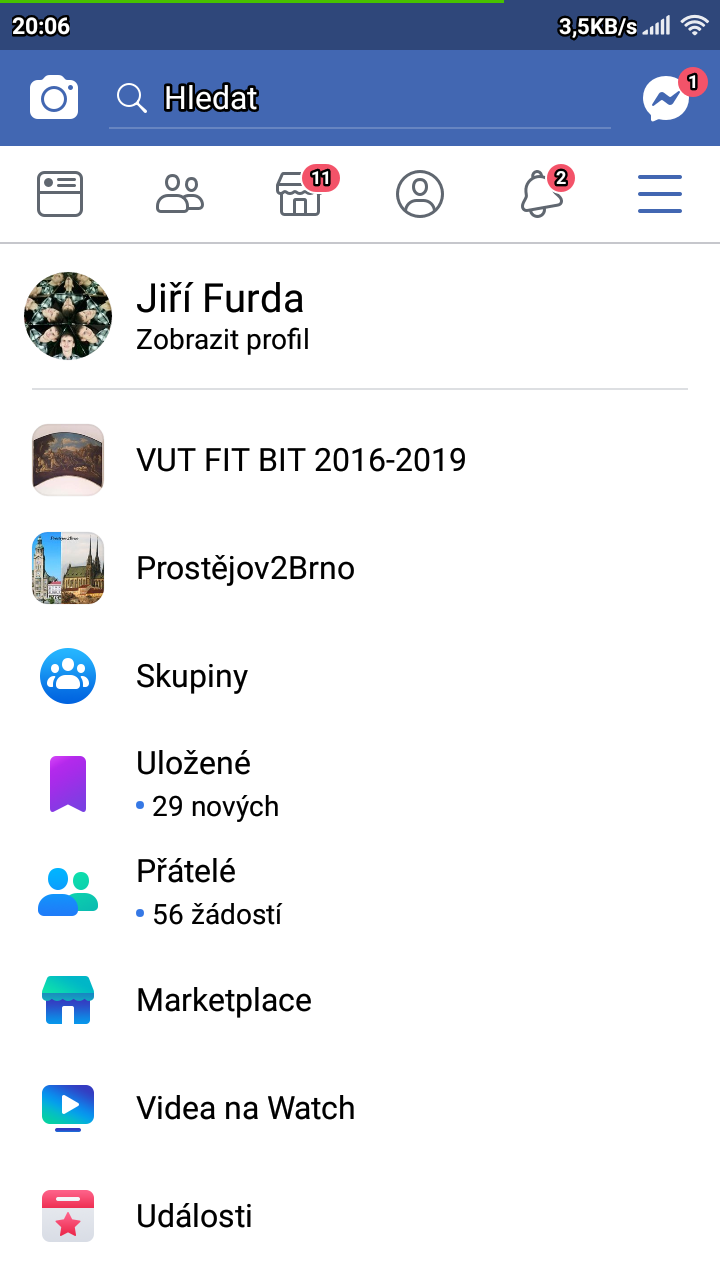
\includegraphics[width=0.5\textwidth-0.4cm]{obrazky-figures/fb-hamburger-2.png}
	\caption{Hamburgerové menu použité v~mobilní aplikaci sociální sítě Facebook\protect\footnote{Mobilní aplikace Facebook v~obchodě Google Play: \url{https://play.google.com/store/apps/details?id=com.facebook.katana&hl=cs}}. Jeho zobrazení je ovládáno tlačítkem v horní pravé části obrázků, znázorněným třemi vodorovnými čárami. Na levém snímku je možné vidět aplikaci se skrytým menu a v pravém snímku zase se zobrazeným.}
	%TODO zakryt jmeno
\end{figure}



\subsection{Princip nejdříve mobil}\label{section:mobile-first}
Ustálenou technikou, jak vyvíjet responzivní design webových stránek, je princip \uv{nejdříve mobil} (anglicky \emph{mobile-first}). Jak název vypovídá, základní myšlenkou tohoto principu je nejdříve myslet na mobilní zařízení, a až poté na desktopová zařízení. Tento přístup je možné aplikovat jak pro samotný návrh designu, tak i~pro jeho následnou implementaci.

Protože mobilní zařízení nabízejí o~mnoho menší zobrazovací plochu než desktop, je zde každý kus prostoru drahocenný. Designér si proto musí nejprve ujasnit, které části webové stránky jsou pro uživatele prioritní a na základě těchto priorit sestavit návrh.

V~případě využití tohoto principu při samotné implementaci designu se postupuje obdobně. Pokud jsou všechny kaskádové styly jak pro mobilní, tak pro desktopová zařízení zapsána v~jednom souboru, bude tento soubor na začátku nejprve obsahovat styly společné pro obě zařízení a styly určené pouze pro mobilní zařízení. Až poté se budou v~souboru objevovat specifické styly, nejpravděpodobněji podmíněné hodnotou vlastnosti \texttt{min-width}. Tyto styly budou aplikovány od určité šířky displeje a budou zaměřené na zobrazení například v desktopových zařízeních. Díky tomuto přístupu bude samotný kód stylů zjednodušen. U~mobilních zařízení bývá zpravidla potřeba méně stylů a často lze využít některé z~výchozích vlastností daných prvků~\cite{bib:mobile-first}.


\section{Boostrap}
\emph{Tato kapitola čerpá z~\cite{bib:bootstrap}}.

Bootstrap\footnote{Bootstrap: \url{https://getbootstrap.com/}} je systém pro snadný vývoj klientské části webových stránek. Je vyvíjen společností Twitter\footnote{Twitter: \url{https://twitter.com/}}, která jej v~roce 2010 vydala jako otevřený software. Jen dva roky poté se Bootstrap stal nejoblíbenějším projektem na stránce GitHub\footnote{GitHub: \url{https://github.com/}}. Bootstrap se skládá převážně z~kaskádových stylů, ale interaktivní prvky využívají skriptovací jazyk JavaScript s~knihovnou jQuery\footnote{jQuery: \url{https://jquery.com/}}. Existují ovšem i další alternativy, které místo jQuery využívají například Vue.js\footnote{BootstrapVue: \url{https://bootstrap-vue.js.org/}}, React\footnote{React Bootstrap: \url{https://react-bootstrap.github.io/}} nebo Angular\footnote{NG Bootstrap: \url{https://ng-bootstrap.github.io/\#/home/}}.

Bootstrap se drží moderních zásad jako princip \uv{nejdříve mobil} (uvedený v~kapitole~\ref{section:mobile-first}) a nabízí snadnou možnost tvorby responzivního designu (popsaného v~kapitole~\ref{section:responsive}). Mimo to také nabízí možnost využít moderně působící vzhled základních HTML prvků jako jsou například vstupní pole formuláře nebo tlačítka. Bootstrap ale poskytuje i~celou řadu nových předpřipravených komponent, a to ku příkladu karty, modální okna, stránkování, informační hlášky a spoustu dalších.

Vzhledem ke své rozsáhlé komunitě lze nalézt mnoho dalších uživateli tvořených komponent nebo dokonce celých hotových šablon webů postavených na tomto systému. Jedna ze stránek, určená pro sdílení takového obsahu, se nazývá Bootsnipp\footnote{Bootsnipp: \url{https://bootsnipp.com/}}.



\section{Python}
Python\footnote{Python: \url{https://www.python.org/}} je vysokoúrovňový interpretovaný objektově orientovaný programovací jazyk. Byl vytvořen roku 1990 a jeho autorem je \emph{Guido van Rossum}. Samotné jádro tohoto jazyka je velmi malé, ale nabízí využití spousty nástrojů pro celou řadu nejrůznějších účelů, psaných jak v~samotném Pythonu tak i~v jazyce C nebo C++~\cite{bib:python}. Specifikem tohoto jazyka je nepoužívání středníku jako oddělovače instrukcí a také striktní pravidla pro odsazení kódu. Podle odsazení se totiž rozlišují bloky kódu, na rozdíl od většiny ostatních jazyků, kde k tomuto účelu slouží symboly složených závorek. 


\subsection{Flask}
Flask\footnote{Flask: \url{http://flask.pocoo.org/}} je systém s otevřeným zdrojovým kódem určený pro tvorbu systémové části webových stránek. Tento systém je napsaný v~programovacím jazyce Python a jedná se o systém typu \emph{micro-framework}. Klíčový znak tohoto typu systémů je co nejmenší nebo i~nulová závislost na externích knihovnách~\cite{bib:flask-doc}.
Flask si klade za cíl udržet co nejjednodušší jádro, ale zároveň se soustředí na možnost tento základ jednoduše rozšířit~\cite{bib:flask-pym}.

Smyslem systému Flask je být základním kamenem pro jakýkoliv typ webové aplikace. Z~tohoto důvodu na rozdíl od ostatních systémů neobsahuje žádnou abstrakci databázové vrstvy nebo knihovnu pro formuláře. V případě potřeby využití takovýchto funkcí, lze použít některé z~dostupných rozšíření~\cite{bib:flask-design}.

Ve svém základu systém využívá šablonovací jazyk Jinja2\footnote{Jinja2: \url{http://jinja.pocoo.org/}} zjednodušující udržení konzistentní struktury stránek. Poskytuje například dědičnost šablon nebo znovupoužitelné bloky a dokáže se vypořádat s~bezpečnostními útoky typu XSS (\emph{Cross Site Scripting})~\cite{bib:jinja}.
Druhou knihovnou, kterou systém Flask využívá, je Werkzeug\footnote{Werkzeug: \url{https://pypi.org/project/Werkzeug/}} - jedna z~nejpokročilejších knihoven pro rozhraní brány webového serveru (WSGI neboli \emph{Web Server Gateway Interface}), které umožňuje webovou aplikaci provozovat nezávisle na technologii použité na serveru~\cite{bib:flask-pep}.

Tento systém je využíván například sociální sítí Pinterest\footnote{Pinterest: \url{https://cz.pinterest.com/}}~\cite{bib:flask-pinterest}
nebo síťovou dopravní společností Lyft\footnote{Lyft: \url{https://www.lyft.com/}}~\cite{bib:flask-lyft}.



\section{Vue.js}\label{section:Vue.js}
V~dnešní době jsou webové prohlížeče stále schopnější a výkonnější. Díky tomu se stává trendem přenášet stále větší části webové aplikace ze serveru na stranu klienta. Toho je docíleno pomocí programovacího jazyku JavaScript. V~současné době se nejvíce využívá knihovna jQuery, %[Todo: najít zdroj]
ale začali se objevovat pokročilejší systémy jako například React\footnote{React: \url{https://reactjs.org/}}, Angular\footnote{Angular: \url{https://angular.io/}} a v~neposlední řadě Vue.js\footnote{Vue.js: \url{https://vuejs.org/}}.

Vue.js je progresivní systém - přizpůsobuje se složitosti projektu. Podobně jako dříve zmiňovaný systém Flask se nejedná o~rozsáhlý systém, jehož části by se vypínaly, ale jedná se o~základní systém, který lze dále rozšiřovat~\cite{bib:vue-progressive}.
Díky tomuto přístupu učební křivka není tak strmá, jako u~konkurenčních systémů. Jediné, co člověku pro začátek práce se systémem Vue.js stačí, je být obeznámen s~jazyky HTML a JavaScript~\cite{bib:vue-curve}.

Jedna z~předností toto systému je jednoduchost obousměrné vazby dat. Tato vazba znamená, že hodnota proměnné v~jazyce JavaScript je synchronizována s~hodnotou v~objektovém modelu dokumentu (DOM neboli \emph{Document Object Model}) a to stejné platí i~v~opačném směru~\cite{bib:vue-binding}.
V~praxi může být tato funkce využita například v~internetovém obchodě, kdy uživatel klikne na tlačítko \uv{Přidat do košíku}, které pouze rozšíří pole košíku o~další produkt. Bez jakéhokoliv dalšího úsilí komponenty, závislé na této proměnné zaznamenají změnu a automaticky provedou odpovídající akce - košík přepočítá celkový počet vybraného zboží, celkovou cenu nákupu, zlevní se cena daného produktu, při koupi dalších kusů apod. 


\subsection{Vue Router}
Mezi oficiálně podporované knihovny patří například Vue Router\footnote{VueRouter: \url{https://router.vuejs.org/}}, umožňující tvorbu jednostránkové aplikace, kdy se načte pouze jedná jediná stránka a pomocí jazyku JavaScript a asynchronních požadavků se mění části obsahu webu. Server v~takovém případě slouží pouze jako úložiště dat a veškerou prezentaci se stará strana klienta~\cite{bib:vue-router}. %TODO obsahuje pekny ilustrace


\subsection{Vuex}
Dalším oficiálním rozšířením je Vuex, knihovna pro správu stavu. Pokud se v~aplikaci používá více komponent, které využívají stejnou proměnnou, brzy se zdrojový kód stává neudržitelným. 
V~tuto chvíli je vhodné využit knihovnu Vuex. Jejím účelem je udržovat centrální stav proměnných, které jsou sdíleny napříč různými komponentami v~aplikaci. Tohoto je docíleno díky dodržování návrhového vzoru jménem Flux~\cite{bib:vuex-doc}. 
%TODO: Reference na MVC -> WTF?


\subsubsection*{Návrhový vzor Flux}
\emph{Tato kapitola čerpá z~\cite{bib:vuex-guide}}.

Mezi základní pilíře návrhového vzoru Flux patří několik následujících pravidel, kterých se knihovna Vuex drží. Principy fungování tohoto návrhového vzoru jsou vyobrazeny v~diagramu~\ref{img:vuex-dataflow}.

\begin{itemize}
    \item \textbf{Jediný zdroj pravdy.} Data, která jsou sdílena více komponentami, jsou uložena na jednom místě - sklad (anglicky \emph{store}) a jsou oddělena od komponent, které je využívají. Komponenty mohou stále mít svá lokální data, ale nesmějí mít svou kopií sdílených dat, ty se vždy musí číst ze skladu.
    \item \textbf{Data pouze ke čtení.} Komponenty nesmějí přímo upravovat data ve skladu. V~případě potřeby změny těchto dat sklad pouze informují a ten se sám o~postará o~provedení změny pomocí tzv.~mutací (Reprezentovány uzlem \emph{Mutations} v~grafu \ref{img:vuex-dataflow}). Díky tomu se minimalizuje šance nepředpokládaných změn těchto dat a funkce, starající se o~tyto změny jsou jednodušeji dohledatelné.
    %TODO: AddToCart mutation example?
    \item \textbf{Změny dat jsou synchronní.} Asynchronní provádění operací mnohdy přináší spoustu výhod, v~tomto případě je ale vyžadováno mutace provádět synchronně kvůli odstranění závislosti na pořadí a načasování různých událostí.
\end{itemize}

\begin{figure}[H]
	\centering
	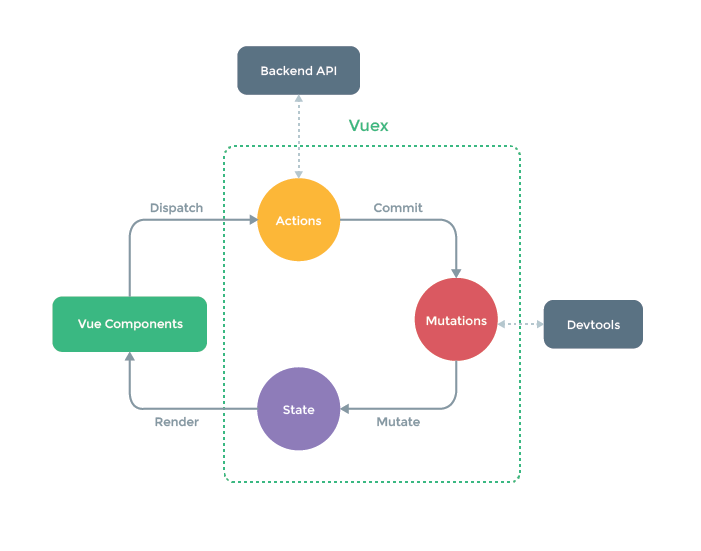
\includegraphics[width=\textwidth]{obrazky-figures/vuex.png}
	\caption{Diagram znázorňující životní cyklus dat v~knihovně Vuex. \emph{Převzato z~\cite{bib:vuex-doc}}}
	%TODO: Popsat v obrázku nebo v textu?
	\label{img:vuex-dataflow}
\end{figure}

\blindtext


\subsubsection*{BootstrapVue}
\emph{Tato kapitola čerpá z~\cite{bib:bootstrap-vue}}.

BoostrapVue je systém klientské části webových stránek založený na systému Bootstrap, který pro svou plnou funkčnost vyžaduje použít také knihovnu jQuery. Pokud ale webová aplikace již pracuje se systémem Vue.js, mnohdy odpadá potřeba jQuery v~aplikaci využívat. Vzhledem k~tomu, že se jedná o~poměrně rozsáhlou knihovnu, není žádoucí ji používat jen z~důvodu, že je aplikace postavená na systému Bootstrap.

V~tuto chvíli je vhodné použít alternativu jménem BoostrapVue, která závislost na knihovně jQuery nahrazuje závislostí na systému Vue.js. Systém BootstrapVue nabízí všechny komponenty původního systému, některé dokonce vylepšuje a také nabízí komponenty úplně nové.

Mimo to využití této knihovny také přináší větší pohodlí pro vývojáře. Dlouhý zápis některých komponent, tvořených pomocí množství vnořených prvků \texttt{<div>} lze díky Vue.js značně zjednodušit. Dokáže totiž prvek struktury HTML nahradit za rozsáhlejší strukturu na základě šablony komponenty. Konvencí systému je takové prvky pojmenovávat s~předponou \texttt{b-}, například tedy \texttt{b-button}.
Přímo učebnicovým příkladem takového zjednodušení je zápis modálního okna, které se klasickým způsobem tvoří následovně:

\begin{verbatim}
<div class="modal" tabindex="-1" role="dialog">
  <div class="modal-dialog" role="document">
    <div class="modal-content">
      <div class="modal-header">
        <h5 class="modal-title">Modal title</h5>
        <button type="button" class="close" data-dismiss="modal"
        aria-label="Close">
          <span aria-hidden="true">&times;</span>
        </button>
      </div>
      <div class="modal-body">
        <p>Modal body text goes here.</p>
      </div>
      <div class="modal-footer">
        <button type="button" class="btn btn-secondary"
        data-dismiss="modal">Close</button>
        <button type="button" class="btn btn-primary">Save changes</button>
      </div>
    </div>
  </div>
</div>
\end{verbatim}
\emph{Kód byl převzat z~\cite{bib:bootstrap-modal}}

Pomocí BoostrapVue lze identickou komponentu zapsat mnohem elegantnějším způsobem a to konrkétně:

\begin{verbatim}
<b-modal title="Modal title">
  <p>Modal body text goes here.</p>
</b-modal>
\end{verbatim}




\section{Elasticsearch}
\emph{Tato kapitola čerpá z~\cite{bib:elastic-defnitive}}.

Elasticsearch\footnote{Elasticsearch: \url{https://www.elastic.co/products/elasticsearch}} je vyhledávač s otevřeným zdrojovým kódem umožňující distribuované vyhledávání a analýzu v~reálném čase. Umožňuje velmi rychle pracovat s~rozsáhlými daty (anglicky \emph{big data}) a provádět nad nimi plnotextové vyhledávání, strukturované vyhledávání a nebo zmiňovanou analýzu.

Tento vyhledávač je hojně využíván jak menšími projekty, tak i~světoznámými organizacemi. Za zmínku stojí například internetová encyklopedie Wikipedia\footnote{Wikipedia: \url{https://www.wikipedia.org/}}, britský deník The~Guardian\footnote{The Guardian: \url{https://www.theguardian.com/international}}, komunitní stránka pro výměnu rad programátorů StackOverflow\footnote{StackOverflow: \url{https://stackoverflow.com/}} nebo populární webová služba pro verzovací nástroj Git\footnote{Git: \url{https://git-scm.com/}} a to GitHub.

Elasticsearch je postavený na knihovně Apache Lucene\footnote{Apache Lucene: \url{https://lucene.apache.org/}}, využívá především její funkce plnotextového vyhledávání, ale oproti této knihovně samotné Elasticsearch nabízí o~mnoho přívětivější způsob používání, především pro začínající uživatele. 

Jedná se o~bezschémovou databázi, oproti relačním databázím nenabízí propojovací dotazy, a proto je nutné ukládaná data denormalizovat.

\subsection{Základní struktura}
\emph{Tato kapitola čerpá z~\cite{bib:elastic-concept}}.

Základní struktura databáze Elasticsearch se na první pohled od tradičních relačních databázi velmi neliší, ke spoustě pojmů užívaných v databázi Elasticsearch lze nalézt ekvivalent právě z~tohoto typu databází.

\subsubsection*{Uzel a shluk}
Pod pojmem uzel (anglicky \emph{node}) se skrývá server, ve kterém jsou uložena data. Uzel v~rámci databáze může být jeden nebo jich může být i~více a každý bude obsahovat pouze určitou část dat. Tyto uzly jsou seskupeny do shluku (anglicky \emph{cluster}).

\subsubsection*{Dokument}\label{section:dokument}
Dokument je základní jednotka dat, které může být zaindexována. Obsah dokumentu je zapsán ve formátu (anglicky \emph{JavaScript Object Notation}). V~relační databázi lze dokument přirovnat k~řádku tabulky.

\subsubsection*{Index}\label{section:index}
Skupina dokumentů s~podobnou strukturou se nazývá index. Ekvivalentem v~relačních databázích by v~tomto případě byla tabulka.

\subsubsection*{Střepy}
Elasticsearch nabízí možnost index rozdělit na střepy (anglicky \emph{shards}), které mohou být uloženy v~různých uzlech. Tuto možnost je vhodné využít především při práci s~indexy s~velkým obsahem dat. Díky rozdělení docílíme distribuování zátěže a lze využít paralelní zpracování, tudíž bude zpracování dotazu odbaveno výrazně rychleji. 
Přístup k~takto rozděleným indexům se nijak nemění a pro uživatele je tento proces naprosto transparentní.

\subsubsection*{Repliky}
Obdobně lze využít i~repliky. Zde se ovšem data indexu nerozdělují, ale naopak duplikují. Díky uložení těchto replik mezi více uzly může systém být robustnější a dokáže fungovat i~v~případě selhání části shluku. I~v~tomto případě je umožněno vyhledávat paralelně. 

\subsection{Dotazy}
Pro komunikaci s~touto databází se využívá Query DSL - dotazy aplikačního rozhraní REST (anglicky \emph{Representational State Transfer}) ve formátu JSON.

Obsah dotazu může vypadat například následovně:
\begin{verbatim}
{
  "query": { 
    "bool": { 
      "should": [
        { "match": { "title": "Virtual Reality" }}, 
        { "match": { "title": "Augmented Reality" }}  
      ],
      "filter": [ 
        { "term":  { "participant.country.keyword": "Czech Republic" }}
      ]
    }
  }
}
\end{verbatim}

\blindtext

Na tento dotaz můžeme server odpověď zprávou s~obsahem:

\begin{verbatim}
{
  "took" : 38,
  "timed_out" : false,
  "_shards" : {
    "total" : 5,
    "successful" : 5,
    "skipped" : 0,
    "failed" : 0
  },
  "hits" : {
    "total" : 1515,
    "max_score" : 15.635861,
    "hits" : [
      {
        "_index" : "xstane34_projects",
        "_type" : "data",
        "_id" : "101785",
        "_score" : 15.635861,
        "_source" : {
          "startDate" : "2012-01-01",
          "endDate" : "2015-12-31",
          "reference" : "278169",
    ...
\end{verbatim}

\blindtext


\subsubsection*{Kontext}
\emph{Tato kapitola čerpá z~\cite{bib:elastic-context}}.

Dotazy v~Elasticsearch se rozlišují na dva základní typy - kontext dotazu (\emph{query}) a kontext filtru.

První z~nich se dá lidsky přeložit do otázky \uv{Jak moc dokument splňuje dotaz?}. V~tomto případě se u~každého výsledku počítá skóre relevance, podle kterého jsou ve výsledné odpovědi dokumenty sestupně řazeny.

Druhý typ dotazů, jak název vypovídá, je určen především k filtrování. V lidské řeči by se tento typ dotazů formulovat jako \uv{Splňuje dokument dotaz?}. Vyhodnocení tohoto typu dotazů je mnohem rychlejší, díky absence nutnosti počítat skóre relevance. Mimo to jsou takovéto dotazy automaticky ukládány do mezipaměti, což výrazně urychluje jejích opětovné využití. 

V jednom složeném dotazu je možné oba tyto typy kombinovat.

\subsection{Metadata}
\blindtext

\subsection{Fasetové vyhledávání}
S~velkým množstvím dat přichází potřeba obsah podle určitých kriterií zúžit. K~tomutu účelu slouží filtry a fasetové vyhledávání (někdy také označována jako fastová navigace - anglicky \emph{faceted search} nebo \emph{faceted navigation}). Využití faset je ale pokročilejší než použít filtry, protože fasetová navigace umožňuje využít hned několik filtrů najednou~\cite{bib:facet}.

V~Elasticsearch je možné tuto navigaci vytvořit pomocí tzv.~kyblíkových agreagací (angl. \emph{bucket aggregations}).
Jednoduše řečeno, se pro dokumenty vytvoří kyblíky, kde každý z~kyblíku odpovídá určitému kriteriu. Pokud dokument toto kriterium splňuje, je do kyblíku vložen~\cite{bib:elastic-bucket}.

S~tímto typem vyhledávání se lze setkat velmi často v~seznamech produktů například v~internetových obchodech nebo cenových srovnávačích.

\begin{figure}[H]
	\centering
	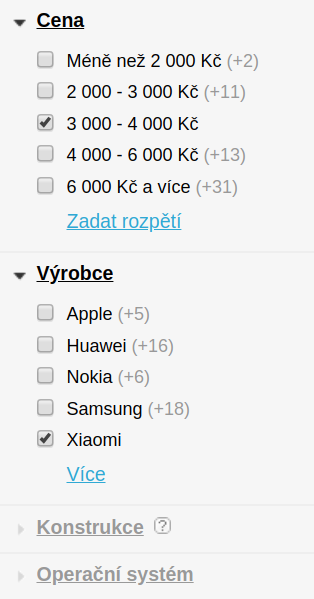
\includegraphics[width=0.35\textwidth]{obrazky-figures/heureka-facet.png}
	\hspace{0.5cm}
	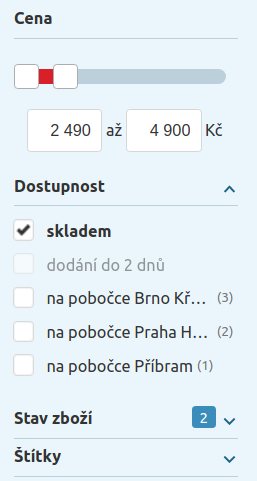
\includegraphics[width=0.35\textwidth]{obrazky-figures/czc-facet.png}
	\caption{Příklad využití fasetového vyhledávání na cenovém srovnávači Heureka\protect\footnote{Heureka: \url{https://www.heureka.cz/}} (vlevo) a internetovém obchodě CZC.cz\protect\footnote{CZC.cz: \url{https://www.czc.cz/}} (vpravo).}
\end{figure}


\subsection{Plnotextové vyhledávání}
\emph{Tato kapitola čerpá z~\cite{bib:elastic-defnitive}}.

Uložená data se dělí na dva typy - přesné hodnoty a plnotextové hodnoty (anglicky \emph{full-text}). Přesné hodnoty jsou určeny pro data, jako například identifikátor uživatele. Pokud totiž vyhledáváme uživatele s~identifikátorem \uv{42}, jako výsledek neočekáváme uživatele, který má identifikátor \uv{420}, ale očekáváme výsledek, který bude přesně splňovat hledanou položku.
Pokud ale člověk pracuje s~textovými položkami, nemusí nutně hledat stoprocentní shodu. Lidský jazyk je velice rozmanitý a umožňuje slova časovat, skloňovat, či vyjádřit jednu věc vícero synonyma. %todo sklonuju spravne?
V~těchto případech hledání totožných hodnot selhává, i~když má text z~pohledu člověka stejný nebo podobný význam. Pro tento typ hledání slouží právě plnotextové hledání. Můžeme se s~ním setkat například při hledání článku v~internetovém magazínu.
Elasticsearch pro takové hledání musí text nejprve analyzovat a vytvořit pro něj obrácené indexy.

\subsubsection*{Obrácený index}
Obrácený index (anglicky \emph{inverted index}) je datová struktura obsahující seznam všech unikátních slov vyskytujících se v~uložených dokumentech. Pro každé z~těchto slov uchovává informaci, ve kterých dokumentech se vyskytovalo. Díky tomu je možné v~textových položkách rychle provádět plnotextové hledání.

Příkladem mohou být dva dokumenty, kde každý obsahuje právě jednu z~následujících vět:
\begin{itemize}
    \item Na moskevském letišti se stala havárie letadla.
    \item Moskvu silně zasáhla včerejší havárie na letišti.
\end{itemize}
Zpracováním těchto dvou dokumentů tedy může vzniknout následující obrácený index:


\begin{table}[h!]
\centering
\begin{tabular}{ |l|c|c| } 
\hline
Token & Dokument č. 1 & Dokument č. 2 \\
\hline
Moskvu & Ne & Ano \\
Na & Ano & Ne \\
havárie & Ano & Ano \\
letadla & Ano & Ne \\
letišti & Ano & Ano \\
moskevském & Ano & Ne \\
na & Ne & Ano \\
se & Ano & Ne \\
silně & Ne & Ano \\
stala & Ano & Ne \\
včerejší & Ne & Ano \\
zasáhla & Ano & Ne \\
\hline
\end{tabular}
\caption{Ilustrační příklad obraceného indexu pro dva dokumenty.}
\end{table}

Takovýto index by byl ale v~praxi nepoužitelný. Hledání slova \uv{havárie} by sice za výsledek označilo oba dva dokumenty, ale ku příkladu hledání fráze \uv{letiště Moskva} by v tomto případě nenalezlo žádnou shodnu i~když z~lidského pohledu se oba dva dokumenty hledané fráze týkají. Z tohoto důvodu text nestačí pouze strojově rozdělit do tokenů, ale musí proběhnout kompletní analýza textu.

\subsubsection*{Analýza}
Analýza představuje proces, kdy se kus textu rozdělí do jednotlivých tokenů a následně se tyto tokeny upraví do podoby vhodné pro použití plnotextového vyhledávání. Tento proces obstarává analyzér, který se skládá ze tří části:
\begin{itemize}
    \item \textbf{Filtry znaků} upraví zpracovávaný řetězec ještě před samotným rozdělením do tokenů. Jeho úkolem může například být odstranění HTML značek z~textu.
    \item \textbf{Tokenizér} z~textu sestaví jednotlivé tokeny. Tokeny ve většině případů představují jednotlivá slova, ale nemusí tomu tak vždy být. 
    \item \textbf{Filtry tokenů} na konec projde všechny vytvořené tokeny, může některé odstranit, přidat a nebo jen upravit. 
\end{itemize}
Filtrů může být v~jednom analyzéru použitá celá řada a to jak filtrů znaků, tak i~filtrů tokenů. Tokenizér je ale v~rámci analyzéru vždy použit jen jeden jediný.

Elasticsearch již ve svém základu nabízí škálu různých analyzéru. Tyto analyzéry jsou různé složitosti, mezi ty nejjednodušší patří analyzér bílých znaků, který text rozdělí striktně podle mezer, tudíž je i~tečka na konci věty vnímána jako část slova. Nejčastěji se ale člověk může setkat s~jazykovým analyzérem, který je uzpůsoben lidské řeči. Elasticsearch takový analyzér nabízí pro mnoho jazyků mezi které patří i~jazyk český.

\subsubsection*{Filtry tokenů}
\emph{Tato kapitola čerpá z~\cite{bib:elastic-fulltext}}.

Velmi častou filtrací bývá změna velkých písmen na malé, díky tomu nejsou slova na začátku věty vnímána jako jiná slova, než ty v~jiné části věty. Pro český jazyk je také typické odstranění diakritiky.

Součástí analyzátorů bývá často odstranění tokenů, které obsahují nepodstatná slova. Jedná se především o~spojky a předložky. Taková slova se v~plnotextovém vyhledávání označují jako \emph{stop slova} (anglicky \emph{stop words}). Tento seznam je vždy specifický pro konkrétní jazyk textu, použít výchozí anglická stop slova nad česky psaným textem by ztrácelo význam.

Další nedílnou součástí pokročilejších analyzátorů je \emph{stematizace}, aneb získání kmene slova. Pro tuto operaci lze využit dva způsoby a to algoritmus nebo slovník. Každý z~těchto způsobů má své pro a proti.
Využitím algoritmické stematizace sice analyzátor nemusí znát všechna slova v~daném jazyce, protože slova převádí do požadovaného tvaru pouze na základě sady pravidel, ale zase dochází k~určité nepřesnosti. Elasticsearch v~případě využití české algoritmické stematizace ze slov odstraňuje všechny přípony.
Druhým způsobem, který lze využít je stematizace na základě slovníku. Díky tomu jsou převedené tvary přesnější než ty získané algoritmem, ale hlavním předpokladem je využití vhodného slovníku s~dostatečnou zásobou slov.
%TODO priklad

\subsection{Podobnostní hledání}
\blindtext[2]

\subsection{Knihovny}
Elasticsearch také vyvíjí několik oficiálně podporovaných nízkoúrovňových klientů pro mnoho populárních programovacích jazyků. Patří mezi ně například Java, JavaScript, Go, .NET, PHP, Perl nebo Python~\cite{bib:elastic-clients}.
Klientů vyvíjených komunitou lze samozřejmě nalézt o~mnoho více\footnote{Komunitní klienti Elasticsearch: \url{https://www.elastic.co/guide/en/elasticsearch/client/community/current/index.html}}.

Práce s~nízkoúrovňovými klienty pro programátory nebývá příliš pohodlná, z~tohoto důvodu vznikají komunitou vyvíjení klienti, kteří nabízí vysokoúrovňový přístup. Konkrétně pro programovací jazyk Python byl do roku 2015 společností Mozilla\footnote{Mozzila: \url{https://www.mozilla.org/}} vyvíjen klient jménem \emph{ElasticUtils}\footnote{ElasticUtils: \url{https://elasticutils.readthedocs.io/en/latest/}}. Za nástupce toho klienta je považována knihovna Elasticsearch DSL\footnote{Elasticsearch DSL: \url{https://elasticsearch-dsl.readthedocs.io/en/latest/}}~\cite{bib:elastic-utils}.

\subsubsection*{Elasticsearch DSL}
\emph{Tato kapitola čerpá z~\cite{bib:elastic-dsl}}.

Elasticsearch DSL je rovněž knihovna pro programovací jazyk Python. Jedná se o~vysokoúrovňovou knihovnu postavenou na oficiální nízkoúrovňové knihovně Python Elasticsearch Client\footnote{Python Elasticsearch Client: \url{https://elasticsearch-py.readthedocs.io/en/master/}}. Díky tomu lze s~dokumenty v~databázi Elasticsearch pracovat jako s~objekty, ale zároveň je stále možné použít původní přístup oficiálního klienta ku příkladu ke zjištění zdraví shluku.

Jako příklad mějme následující dotaz, napsaný s~využitím oficiální knihovny Python Elasticsearch Client:
\begin{verbatim}
from elasticsearch import Elasticsearch
client = Elasticsearch()

response = client.search(
{
  index="xstane34_projects",
  body={
    "query": { 
      "bool": { "must": { "title": "Virtual Reality" }}, 
        "filter": [ 
          { "term":  { "participant.country.keyword": "Czech Republic" }}
        ]
      }
    },
    "aggs": {
        "coordinator_coutry": {
          "terms": {"field": "coordinator.country.keyword"},
        }
      }
  }
\end{verbatim}

Tento poměrně zdlouhavý dotaz lze se stejným výsledkem přepsat za použití knihovny Elasticsearch DSL do následující, mnohem elegantnější formy:

\begin{verbatim}
from elasticsearch import Elasticsearch
from elasticsearch_dsl import Search

client = Elasticsearch()

s = Search(using=client, index="xstane34_projects")  \
    .query("match", title="Virtual Reality")  \
    .filter("term", coordinator__country__keyword="Czech Republic")

s.aggs.bucket("coordinator_coutry", "terms",  \
    field="coordinator.country.keyword")

response = s.execute()
\end{verbatim}
%TODO zkontrolovat

Práce s dotazy je tedy mnohem snadnější a vývojářům alespoň částečně ubývá rutinní činnost. Obrovskou výhodou je sestrojování dotazu pomocí zřetězených funkcí. Díky této funkci knihovny lze dotaz v průběhu programu jednoduše rozšiřovat a kód se tak nemusí stát těžko čitelným.

Objekt dotazu je v knihovně reprezentován třídou \texttt{Search}. Tu lze ale kdykoliv převést do slovníku odpovídajícímu klasickému dotazu ve formátu JSON pomocí metody \texttt{to\_dict()}. Stejně tak je možné dotaz napsaný ve slovníku převést do objektu knihovny Elasticsearch DSL použitím metody \texttt{from\_dict()}. Tato funkcionalita zajišťuje zpětnou kompatibilitu bez nutností zásahu do stávajícího kódu s programy využívajícími například jen nízkoúrovňového klienta Python Elasticsearch Client.



\section{Podobnostní hledání}
Je zvykem uživateli doporučovat další obsah na základě sdílených charakteristik s právě prohlíženým obsahem. Příkladem může být čtení článku na zpravodajském webu.
\blindtext

\subsection{Hledání souvisejících dokumentů}
\blindtext[2]

\subsection{Kontextové procházení kolekcí}
\emph{Tato kapitola čerpá z~\cite{bib:similarity-context}}.



Pro zobrazení relevantnějších výsledků vyhledávání lze využít kontext hledání uživatele. V takovém případě se při počítání skóre relevantnosti nepracuje pouze s aktuálním hledáním, ale i s historií uživatele. Díky tomu je docíleno přizpůsobení výsledků přímo pro daného uživatele.
Pro tyto účely je možné brát v potaz předchozí hledání uživatele nebo podobnost s dříve otevřenými dokumenty.

Výhodou kontextového hledání je zpřesnění výsledků hledání bez nucení uživatele manuálně dané hledání blíže specifikovat. O tuto možnost ovšem uživatel nepřijde, tento typ hledání se s použitím fasetové navigace nijak nevylučuje. 
Mimo to je díky tomuto přístupu možné objevit podobnost i mezi dokumenty, které spolu přímo nesdílí podstatná metadata. 

%shorterm/longterm


\begin{figure}[H]
	\centering
	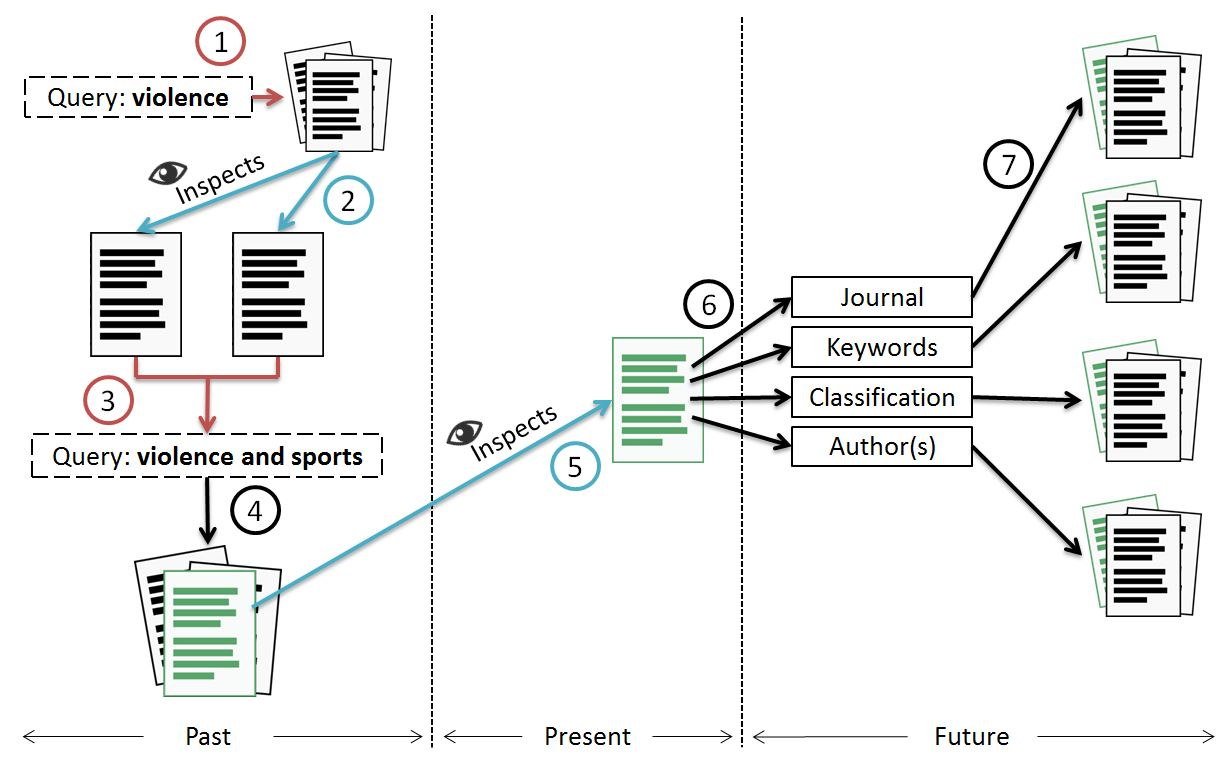
\includegraphics[width=\textwidth]{obrazky-figures/contextual.png}
	\caption{Schéma kontextuálního hledání. Převzato z~\cite{bib:similarity-context}.}
	\label{img:contextual}
\end{figure}

Na obrázku~\ref{img:contextual} uživatel v prvních dvou krocích hledal pojem \uv{violence} a prohlédl si dva výsledky. Poté v kroku 3 hledání rozšířil a vyhledal pojem \uv{violence and sports}. Z výsledků v kroku 4 zvolil dokument, který si zobrazí podrobněji. Tento proces probíhá v současnosti a je reprezentován krokem 5. Krok 6 tvoří kontext pro budoucí hledání. V kroku 7 jsou znázorněna další hledání, kde budou v počítání skóre relevance brána v potaz metadata z právě zobrazeného dokumentu z kroku 5.





\chapter{Návrh a implementace systému}
Tato kapitola popisuje \blindtext

Předchozí řešení mých kolegů umožňovalo vyhledávat pouze projekty a vědecké zprávy. Nabízelo se tento obsah rozšířit o~výzvy k~předkládání návrhů, na základě kterých Evropská komise vybírá projekty, který budou uskutečněny se spolufinancováním Evropské unie.
%[https://ec.europa.eu/info/funding-tenders/opportunities/portal/screen/home 27.4.].
Samotné výzvy jsou ale hodně obecné a zaštiťují mnoho témat napříč různými oblastmi. Dalším úskalím byl nedostatek informací v~popisu výzev. Rozsáhlý slovní popis se vztahovat až ke konkrétním tématům. Proto jsem se rozhodl portál nerozšiřovat o~výzvy, ale právě o~zmiňovaná témata.

\section{Schéma}
Schéma jednotlivých částí systému a jejich návaznost je možné vidět na obrázku~\ref{img:scheme}. Ve vrchní části obrázku jsou znázorněny zdroje dat, které jsou zpracovávány extraktorem dat. Extrakce probíhá bez zásahu správce periodicky za pomoci plánovače úloh (anglicky \emph{cron}). Správce má však možnost extrakci spustit manuálně. Zpracovaná data jsou ukládána do databáze, odkud je čerpá webový portál a následně je prezentuje uživateli. V blocích modulů systému (\uv{databáze}, \uv{extraktor dat} a \uv{webový portál}) jsou znázorněna loga klíčových technologií využitím pro fungování tohoto modulu.

\begin{figure}[H]
	\centering
	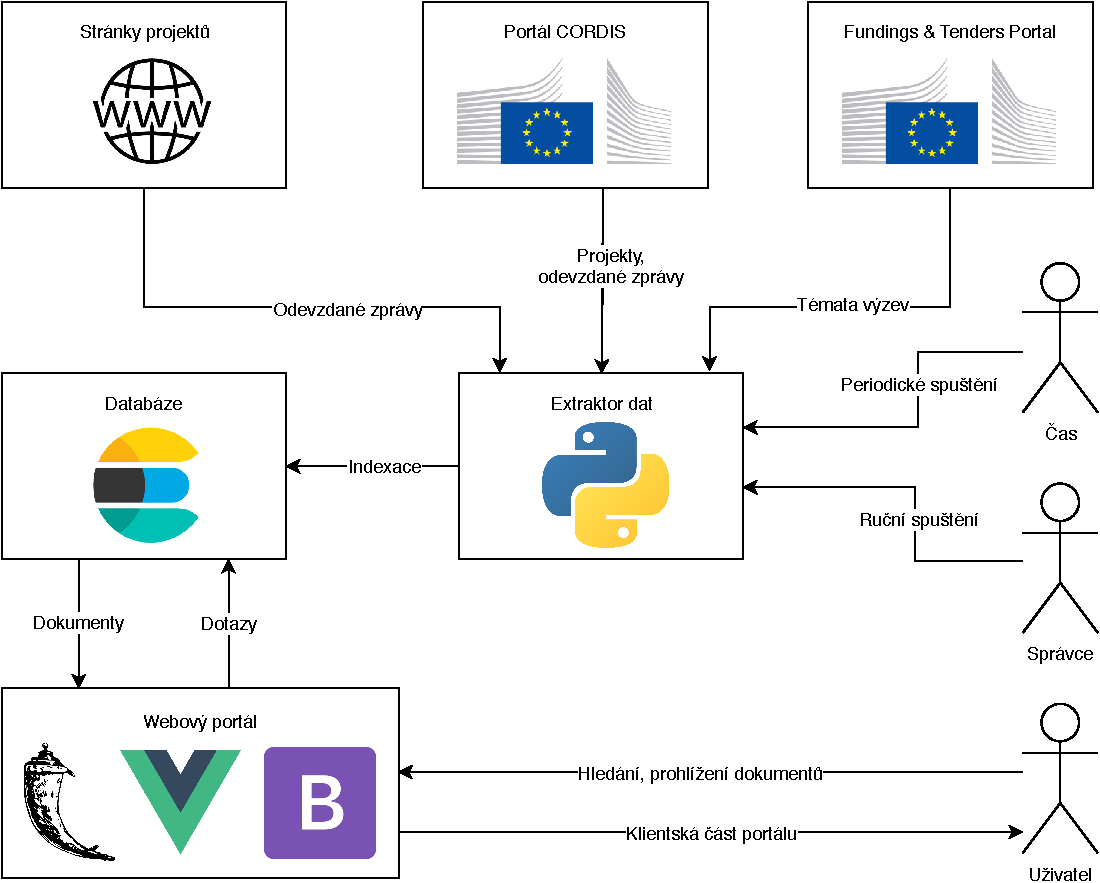
\includegraphics[width=\textwidth]{obrazky-figures/my-scheme.pdf}
	\caption{Schéma jednotlivých částí vyvíjeného systému.}
	\label{img:scheme}
\end{figure}

\section{Extraktor dat}
\blindtext

\subsection{Témata výzev}
Témata výzev jsou čerpána z portálu Fundings and Tenders (představeném v~kapitole~\ref{section:funding}).
Ten pro tyto účely nabízí aplikační rozhraní, kde je možné získat potřebná data ve formátu JSON, čímž bylo značně zjednodušeno jejich dolování. 

Pro indexaci dat z~toho portálu je nejprve použit dotaz pro získání souhrnného seznam témat. Ten je poté extraktorem postupně celý zpracován. Z~toho seznamu lze získat základní informace o~tématech. Pro každé jedno téma je odeslán nový dotaz, který na základě identifikátoru vrátí podrobnější informace vztahující se k~tématu, jako například jeho slovní popis.

\subsubsection*{The Funding \& Tenders Portal}\label{section:funding}

The Funding \& Tenders Portal\footnote{The Funding \& Tenders Portal: \url{https://ec.europa.eu/info/funding-tenders/opportunities/portal/screen/home}} je webový portál spravován převážně Evropskou komisí. Portál zprostředkovává informace určené hlavně expertům a účastníkům v~programech financovaných EU~\cite{bib:funding-about}.
V~případě zájmu o~zažádání financování výzkumu je nutné nejprve prostřednictvím toho portálu najít výzvu k~předkládání návrhů v~odpovídajícím odvětví a dodržet konkrétní postup pro podání žádosti~\cite{bib:funding-find}.

\subsection{Projekty}
\blindtext

\subsubsection*{CORDIS}
CORDIS\footnote{CORDIS: \url{https://cordis.europa.eu/}} (\emph{The Community Research and Development Information Service}) je portál provozovaný Evropskou Unií (dále jen EU) sloužící jako hlavní zdroj výsledků projektů, sponzorovaných v~rámci programů EU pro výzkum a inovaci. Na jednom místě veřejně poskytuje informace jak o~těchto projektech, tak i~o~jejích účastnících, vědeckých zprávách a publikacích~\cite{bib:cordis}.

\subsection{Odevzdávané zprávy}
\blindtext



\section{Webový portál}
\blindtext

\subsection{Návrh}
\blindtext

\subsection{Podoba}
Vizuální struktura vytvořeného webového portálu lze rozdělit do tří hlavních celků - hlavičky, postranního panelu a hlavního obsahu stránky. První dva z~těchto celků jsou určeny pro specifikaci vyhledávání. Aby bylo vyhledávání při procházení portálu vždy dostupné, pozice těchto celků v~desktopovém zobrazení zůstává neměnná i~při rolování zobrazené stránky.

Portál obsahuje obecně dva typy stránek. Prvním typem jsou stránky obsahující výsledky vyhledávání, které lze vidět na snímku~\ref{image:portal-results}. V~případě úspěšného hledání lze z~těchto výsledků pomocí odkazů \uv{View topic} nebo \uv{View project} přejít na detailní stránku konkrétního výsledku. Tento typ stránek ovšem existuje pouze pro témata a projekty. U~odevzdaných zpráv se místo stránky detailu zobrazí přímo daný dokument. Příklad stránky detailu výsledku je vyobrazen na snímku~\ref{image:portal-detail}.

\begin{figure}[H]
	\centering
	
\includegraphics[width=\textwidth]{obrazky-figures/my-results.png}
	\caption{Stránka vytvořeného portálu zobrazující výsledky hledání výzev s klíčovým slovem \uv{robot} v programu \uv{H2020} a podprogramu \uv{E.2.}}.
	\label{image:portal-results}
\end{figure}
\begin{enumerate}
    \item Logo a název portálu se dle konvence nachází v~levém horním rohu. Zároveň funguje jako odkaz na hlavní stránku.
    \item Zbylá část hlavičky obsahuje vyhledávací pole. Do něj může být vložen i~velmi komplexní dotaz, proto byl při návrhu kladen důraz na co největší šířku tohoto pole. Pod tímto polem se nachází odkazy určující jaký typ výsledků je od vyhledávání očekáván.
    \item V~levé části portálu se nachází postranní panel s~fasetovou navigací. Slouží především pro méně pokročilé uživatele portálu, kterým postačí tvořit jednoduché dotazy. Zároveň lze informace v~tomto panelu využít jako přehled informací typu \uv{Které země se nejčastěji podílí na projektech splňujících dané kriteria?}. Postranní panel je podrobněji popsán v~kapitole~\ref{section:sidebar}.
    \item TODO obsah
\end{enumerate}


\begin{figure}[H]
	\centering
	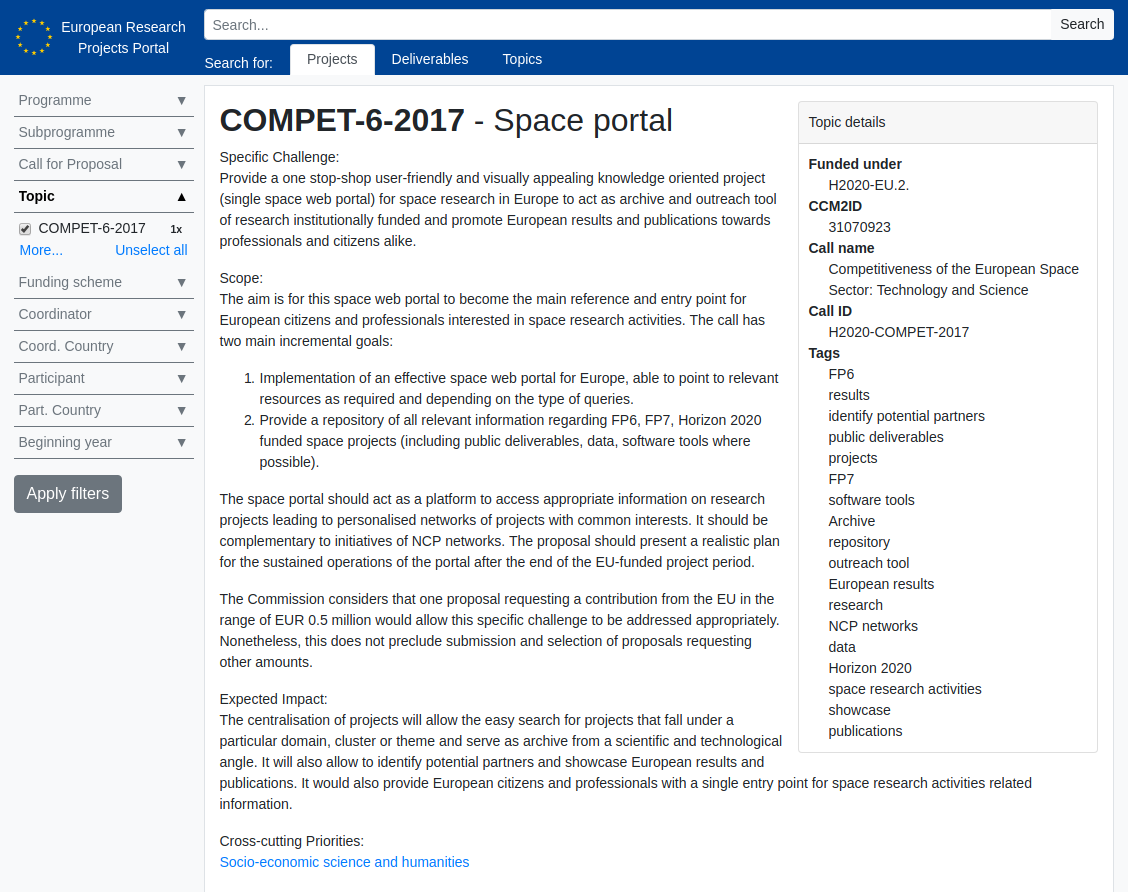
\includegraphics[width=\textwidth]{obrazky-figures/my-topic.png}
	\caption{Snímek vytvořeného portálu zobrazující detailní popis výzvy k předkládání návrhů na téma \uv{Space portal}}.
	\label{image:portal-detail}
\end{figure}
\begin{enumerate}
    \item Plné znění obsahu výzvy a instrukce pro předkládání návrhů na toto téma.
    \item Klíčové specifikace dané výzvy stručně zobrazené v postranní kartě.
    \item Postranní panel s fasetovým vyhledáváním má ve výchozím stavu pro fasetu \uv{Topic} zvolenou možnost právě toho tématu, který je předmětem právě zobrazeného detailu.
\end{enumerate}

\blindtext[2]

\subsection{Struktura adresáře}
Veškeré zdrojové kódy portálu se nachází v~adresáři \texttt{portal}. Uvnitř této složky se nachází adresáře odpovídající architektuře MVC.
\begin{itemize}
  \item Složka \texttt{models} obsahuje modely
  \item Složka \texttt{controllers} obsahuje kontrolery
  \item Složka \texttt{templates} obsahuje pohledy
  \item Složka \texttt{static} obsahuje kaskádové styly a zdrojové kódy Vue komponent
  \item Soubor \texttt{app.py} sloužící ke spuštění portálu
\end{itemize}

\subsection{Vue komponenty}
Některé z~využívaných faset obsahují i~stovky položek a jejich hodnoty mají často dlouhé názvy. Jejich zobrazení pouze v~postranním panelu jsem považoval za nedostatečné, proto jsem se rozhodl toto řešení oproti předchozímu řešení portálu přepracovat s~využitím technologie Vue.js (představenou v~kapitole~\ref{section:Vue.js}) a několika prvků ze systému BootsrapVue. Pro každou z~faset jsem vytvořil dvě komponenty - položku v~postranním panelu a modální okno.

\subsubsection*{Postranní panel}\label{section:sidebar}
Tento panel je tvořen Vue komponentou \texttt{sidebar-facet-list}, která pro každou fasetu vytvoří instanci komponenty \texttt{sidebar-facet}. Několik takových komponent lze vidět na snímku~\ref{img:sidebar}.

Každá komponenta \texttt{sidebar-facet} ve výchozím stavu nabízí nejvýše pět nejčastěji vyskytujících se hodnot dané fasety. Ty jsou postupně nahrazovány zvolenými hodnotami dané fasety. Další hodnoty s~menším výskytem jsou dostupné v~modálním okně, které se zobrazí po kliknutí na tlačítko \uv{\emph{More...}}. Obsahem této komponenty je mimo jiné dílčí komponenta systému BoostrapVue \texttt{b-collapse}, která v~případě potřeby umožňuje danou fasetu minimalizovat. Pokud se takto stane a faseta má zvolené některé ze svých možností, objeví se vedle jejího názvu počet vybraných možností, aby měl uživatel i~při minimalizovaných fasetách přehled o~tom, které možnosti filtrování právě zvolil.

\begin{figure}[H]
	\centering
	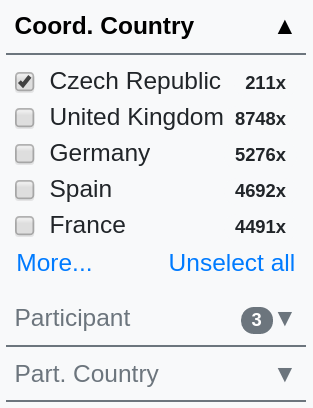
\includegraphics[width=0.3\textwidth]{obrazky-figures/my-facet.png}
	\caption{Část postranního panelu implementovaného portálu}
	\label{img:sidebar}
\end{figure}
%TODO doplnit cisla do obrazku
\begin{enumerate}
    \item Otevřená faseta \uv{Coord. Country} s~jednou zvolenou možností a dalšími čtyřmi nejčastěji vyskytujícími se hodnoty. %TODO vyskytujícími se nebo vyskytujícími-se
    \item Minimalizovaná faseta \uv{Participant} se třemi vybranými možnostmi indikovanými číslem v~pravé části fasety.
    \item Minimalizovaná faseta \uv{Part. Country} bez zvolených možností.
\end{enumerate}


\subsubsection*{Modální okno}
Okna jednotlivých faset jsou tvořena instancemi Vue komponenty \texttt{modal-facet}. O~jejich vytvoření se stará komponenta \texttt{modal-facet-list}. Příklad konkretního modálního okna je možné vidět na snímku~\ref{img:modal}.

Rozsáhlejší výpis možností dané fasety se nyní oproti původnímu řešení portálu zobrazuje v~modálním okně. Zde je možnost současně vidět podstatně více možností a také je možné vypsat jejich hodnoty v~plném znění. V~tomto okně je také obsaženo vstupní pole, které asynchronními dotazy na databázi Elasticsearch vyhledává mezi možnostmi daného fasetu. Samotné modální okno je komponenta systému BootstrapVue, rozšířená o~prvky nutné pro tento portál (například zmiňované vyhledávací pole).

\begin{figure}[H]
	\centering
	
\includegraphics[width=\textwidth]{obrazky-figures/my-modal.png}
	\caption{Modální okno s~dalšími hodnoty fasety s~názvem \uv{Coordinator}}.
	\label{img:modal}
\end{figure}
%TODO doplnit cisla do obrazku
\begin{enumerate}
    \item Nadpis značící, ke které fasetě se modální okno vztahuje.
    \item Vstupní pole pro vyhledávání v~hodnotách fasety.
    \item Fasetové hodnoty odpovídající hledané frázi z~bodu 2. Výsledky se mění v~reálném čase v~závislosti na obsahu tohoto vstupního pole.
\end{enumerate}

\subsubsection*{Fasetová možnost}
Jednotlivé fasetové možnosti jsou reprezentovány komponentou \texttt{option-facet}, která zobrazuje zaškrtávací pole, název dané možnosti a počet výsledků aktuálního vyhledávání obsahující tuto možnost. Při zaškrtnutí možnosti se její data zkopírují do proměnné \texttt{checkedOptions} příslušného fasetu. Tato komponenta se vyskytuje jak v~modálním okně, tak i~v~postranním panelu.

\subsubsection*{Inicializace dat}
Na každé stránce portálu se vyskytuje právě jednou komponenta \texttt{init-facet-data}, která jednorázově obstará naplnění proměnných programovacího jazyka JavaScript.

\subsection{Implementace vyhledávání}
Samotné vyhledávání obstarává třída \texttt{IndexSearch}, při svém vytvoření uloží vstupní parametry a sestaví dotazy pro Elasticsearch. Mezi tyto parametry patří
\begin{itemize}
    \item index, ve kterém se bude hledat
    \item pole dokumentu, ve kterém budou v~případě shody zvýrazněna klíčová slova
    \item pole dokumentu, ve kterých se budou klíčová slova hledat
\end{itemize}
\subsubsection*{buildSearch()}
První z~dotazů je vytvořen tuto metodou, která zpracuje všechny parametry typu GET protokolu HTML a v~případě shody jejich názvů s~některým z~faset, přidá tuto hodnotu do dotazu. Tento dotaz se využívá pro hledání v~modálním okně fasetu. 

\subsubsection*{buildAggregationsSearch()}
Druhý dotaz vzniká rozšířením dotazu z~metody \texttt{buildSearch()}. Je obohacen o~agregaci fasetových hodnot, které jsou poté zobrazeny v~postranním panelu.

\subsubsection*{prepareLayoutData()}
Poté co byly výše zmíněné dotazy vykonány je třeba výsledky zpracovat a připravit pro předání do odpovídajících Vue komponent. Výsledkem této funkce jsou tři struktury JSON, obsahující data využívané pro inicalizaci komponent v~šabloně, zabalení ve slovníku.

Jedna ze struktur, které je poté uložena do skladu knihovny Vuex může vypadat například následovně

\begin{verbatim}
{
    "facets":[
    {
        "mostFrequentOptions":[  
            {  
               "count":8748,
               "text":"United Kingdom",
               "value":"United Kingdom"
            },
            {  
               "count":5276,
               "text":"Germany",
               "value":"Germany"
            },
            ...
         ],
         "field":"coordinator.country.keyword",
         "name":"coordcountry",
         "checkedOptions":[  
            {  
               "count":4692,
               "text":"Spain",
               "value":"Spain"
            },
         ],
         "title":"Coord. Country"
     },
     ...
     ]
}
\end{verbatim}
Každá z~faset má svůj objekt obsažený v~poli s~klíčem \texttt{facets}.
\begin{itemize}
\item \texttt{mostFrequentOptions} obsahuje pole s~nejvýše pěti nejčastějšími hodnotami fasety
%\item \texttt{field} TODO: Už se nepoužívá!
\item \texttt{name} značí unikátní interní název, díky kterému je portál schopný fasetu identifikovat
\item \texttt{checkedOptions} je pole, kde se udržují zvolené hodnoty fasety
\item \texttt{title} nese název fasety, který je zobrazován uživateli
\end{itemize}
Každá z~hodnot faset je zase reprezentována objektem o~třech atributech
\begin{itemize}
\item \texttt{count} udává množství výsledků hlavního hledání s~výskytem této hodnoty fasety
\item \texttt{text} je název hodnoty, která se zobrazuje uživateli
\item \texttt{value} obsahuje reálnou hodnotu, která se aplikuje do dotazu hledání. Od atributu \texttt{text} se mnohdy neliší, ale je třeba mít tyto dvě informace rozdělené například pro použití možností s~názvem sloučených ze dvou polí databáze (příkladem může být název a zkratka instituce)
\end{itemize}

\subsubsection*{createForIndex()}
Protože se v~portálu vytváří hledání na vícero místech, byla vytvořena statická metoda třídy \texttt{IndexSearch}, která vrací předpřipravenou instanci této třidy pro hledání v~jednom z~typů obsahu portálu. Tato funkce očekává ve svém jediném parametru řetězec, určující typ hledání (\texttt{projects}, \texttt{deliverables} nebo \texttt{topics})

\subsubsection*{Hromadné akce}
Pro případy, kdy je potřeba pracovat s~několika hledáními naráz, si lze práci ušetřit využitím dalších statických metod třídy \texttt{IndexSearch} a to konkrétně metoda \texttt{createForEveryIndex()}, která vrací slovník se všemi třemi možnými typy hledání, a poté také \texttt{executeMany()}, která vykoná hledání všech instancí \texttt{IndexSearch} ve slovníku předaném této funkci v~parametru. 

\subsection{Vyhledávání hodnot faset}
Protože ve fasetách lze asynchronně vyhledávat, bylo nutné napsat aplikační rozhraní propojující databázi Elasticsearch s~Vue komponentou reprezentující toto vyhledávání. Tuto činnost obstarává funkce \texttt{showApi} v~kontroleru \texttt{facet\_controller}.

Jako parametr, který je předán cestou URL adresy očekává platný název fasety, pro kterou existuje model třídy \texttt{Facet}. Další parametry jsou předávány metodou GET protokolu HTTP. Prvním povinným parametrem je znění původního dotazu na Elasticsearch, díky tomuto parametru výsledky funkce korespondují s~kontextem aktuálního vyhledávání v~portálu. Dalším parametrem je pak klíčové slovo nebo jeho část, které se hledá v~dostupných hodnotách fasety. 

Po úspěšném dotazu funkce vrací strukturu JSON ve stejném tvaru jako například v~\texttt{checkedOptions} zmiňovaném v~kapitole Vyhledávání %TODO: reference

\subsection{Dotazovací jazyk}
\blindtext[2]

\subsection{Model fasety}
Jednotlivé fasety jsou v portálu implementovány modelovou třídou \texttt{Facet} i přes to, že se jedná o poměrně jednoduché entity, Tento přístup jsem zvolil zejména kvůli větší modulárnosti zdrojových kódů. Metody této třídy jsou většinou statické a usnadňují práci s fasetami napříč portálem.

K vytvoření instance této třídy stačí zadat tři parametry obsahující interní jméno fasety, jméno fasety zobrazované uživateli a také odpovídající pole v dokumentech uložených v databázi Elasticsearch. 

Navázání na pole v databázi je záměrně uváděno bez odpovídajícího indexu. Je předpokladem, že pole použitá pro fasetové vyhledávání jsou ve všech indexech stejně pojmenována. Tento předpoklad umožňuje zachovat zvolené hodnoty fasetového vyhledávání i při přepnutí kontextu hledání. 

Při vytvoření instance se automaticky připraví název toho pole vhodný pro použití jako parametr funkce při sestrojování dotazu (tečky ve vnořených polích je nutné nahradit symboly \texttt{\_\_}). 

\subsubsection*{all()}
Tato statická metoda slouží jako jednotný seznam všech faset dostupných v portálu. Volání metody způsobí vytvoření seznamu obsahující instanci třídy \texttt{Facet} pro všechny dostupné fasety.

\subsubsection*{get()}
Tato třídní metoda se pokusí nalézt odpovídající instanci třídy \texttt{Facet} v seznamu z metody \texttt{all()}. Metoda je využita hlavně při vyhledávání hodnot faset.

\subsubsection*{toDict()}
Jednoduchá metoda převádějící data uvedená v konstruktoru objektu do slovníku. Je určená především k předání informací ze serverové části do Vue komponent v uživatelské části.



\chapter{Experimenty a vyhodnocení}
Tato kapitola popisuje experimenty pro zhodnocení výsledku práce. Část testování byla směřována přímo na uživatele a skládala se jak z implicitní, tak z explicitní zpětné vazby. V závěru kapitoly jsou diskutována možná vylepšení portálu v budoucnu.

\section{Testování na uživatelích}
Do testování portálu se zapojilo TODO uživatelů. Během procházení webového portálu bylo sledováno chování všech těchto uživatelů a následně tato data sloužila pro vytvoření statistik používání. TODO z uživatelů navíc vyplnilo dotazník a tím poskytli přímé sdělení svých dojmů z portálu. 

\subsection{Dotazník uživatelského prožitku}
\emph{Tato kapitola čerpá z~\cite{bib:ueq}}.

Dotazník, zaměřený na uživatelský prožitek (UX neboli \emph{user experience}), se skládal z 26 otázek zaměřených na šest různých aspektů portálu.
\begin{itemize}
    \item \textbf{Atraktivnost} - Celkový dojem.
    \item \textbf{Přesvědčivost} - Je snadné se s ním naučit pracovat?
    \item \textbf{Efektivita} - Lze jej používat bez zbytečného úsilí?
    \item \textbf{Spolehlivost} - Má uživatel pocit, že má vše pod kontrolou?
    \item \textbf{Stimulace} - Je jeho používání vzrušující?
    \item \textbf{Novota} - Je inovativní? Dokáže zaujmout?
\end{itemize}
Tyto aspekty lze rozdělit do dvou skupin. První čtyři uvedené aspekty spadají do skupiny pragmatické kvality, která je zaměřena na technickou efektivnost a splnění cílů. Stimulace a novota jsou oproti tomu aspekty označované jako hedonická kvalita, která je spojovaná s požitkem a potěšením~\cite{bib:hedonic}.

Na všechny otázky bylo možné odpovědět pomocí škály od 1 do 7, přičemž na každé straně škály byly postaveny vzájemně protikladné fráze zaměřené právě na jeden z uvedených aspektů. Respondent pomocí číselné škály volil, ke které frázi mají jeho pocity z portálu blíže.

Obsah dotazníku vycházel z otázek UEQ\footnote{UEQ: \url{https://www.ueq-online.org/}} (\emph{User Experience Questionnaire}) a respondentům byl prezentován pomocí nástroje Google Formuláře\footnote{Google Formuláře: \url{https://www.google.com/intl/cs_CZ/forms/about/}}.

Dotazník vyplnilo TODO repsondentů, nejčastěji se jednalo o muže v období ranní dospělosti. Vzorek účastníku byl složen z pokročilých uživatelů internetu a pouze několik jedinců mělo předchozí zkušenost s portály podobného zaměření. 

% https://www.tablesgenerator.com/
\begin{table}[h!]
\centering
\begin{tabular}{ |l|c|l|l| } 
\hline
Aspekt       & Průměr & Výsledek    & Interpretace                              \\
\hline
Atraktivita  & 1.38   & Nadprůměrný & 25\% výsledků je lepších, 50\% je horších \\
Přehlednost  & 2.06   & Vynikající  & Patří mezi 10\% nejlepších výsledků       \\
Účinnost     & 1.83   & Vynikající  & Patří mezi 10\% nejlepších výsledků       \\
Spolehlivost & 1.71   & Vynikající  & Patří mezi 10\% nejlepších výsledků       \\
Stimulace    & 0.69   & Podprůměrný & 50\% výsledků je lepších, 25\% je horších \\
Originalita  & -0.35  & Špatný      & Patří mezi 25\% nejhorších výsledků       \\  
\hline
\end{tabular}
\caption{Interpretace výsledků dotazníků uživatelského prožitku portálu.}
\label{table:ueq}
\end{table}

\begin{figure}[H]
	\centering
	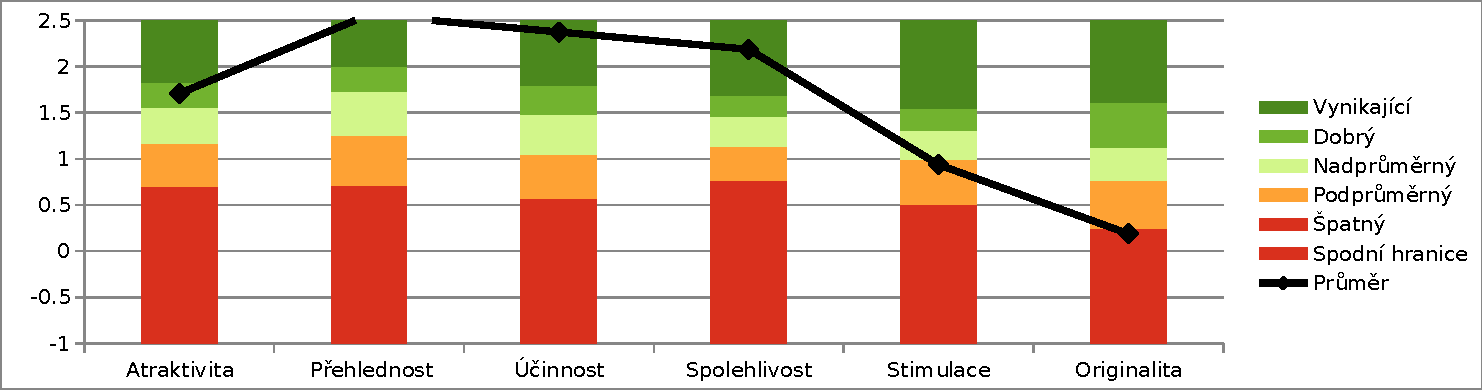
\includegraphics[width=\textwidth]{obrazky-figures/ueq.pdf}
	\caption{Graf prezentující výsledky dotazníků uživatelského prožitku portálu.}
    \label{img:ueq}
\end{figure}

Z výsledků zobrazených v tabulce~\ref{table:ueq} a grafu~\ref{img:ueq} lze usoudit, že většina aspektů portálu je vnímána pozitivně. Za povšimnutí stojí především výborný výsledek v oblasti přehlednosti, což považuji za velký úspěch. Na druhou stranu dotazník odhalil lehce podprůměrné hodnoty v oblasti stimulace a poukázal především na slabou stránku portálu a to jeho originalitu.

V souhrnu lze tedy portál označit jako pragmaticky velmi kvalitní, s podprůměrnou hedonickou kvalitou.
Vzhledem k zaměření portálu ovšem nepovažuji hedonickou kvalitu za tolik podstatnou, proto výsledek uživatelského testování vnímám pozitivně.




\subsection{Sledování chování uživatelů}\label{section:behaviour}
Pro získání analýzy chování uživatelů byl využit nástroj Smartlook\footnote{Smatlook: \url{https://www.smartlook.com/cs/}}. K analýze bylo díky tomu dostupných hned několik typů tepelných map sledujících klikání uživatele, pohyb kurzoru myši nebo rolování po stránce. Navíc bylo možné sledovat nahrávky chování uživatelů a přímo tak pozorovat jejich interakci s portálem.

\begin{figure}[H]
	\centering
	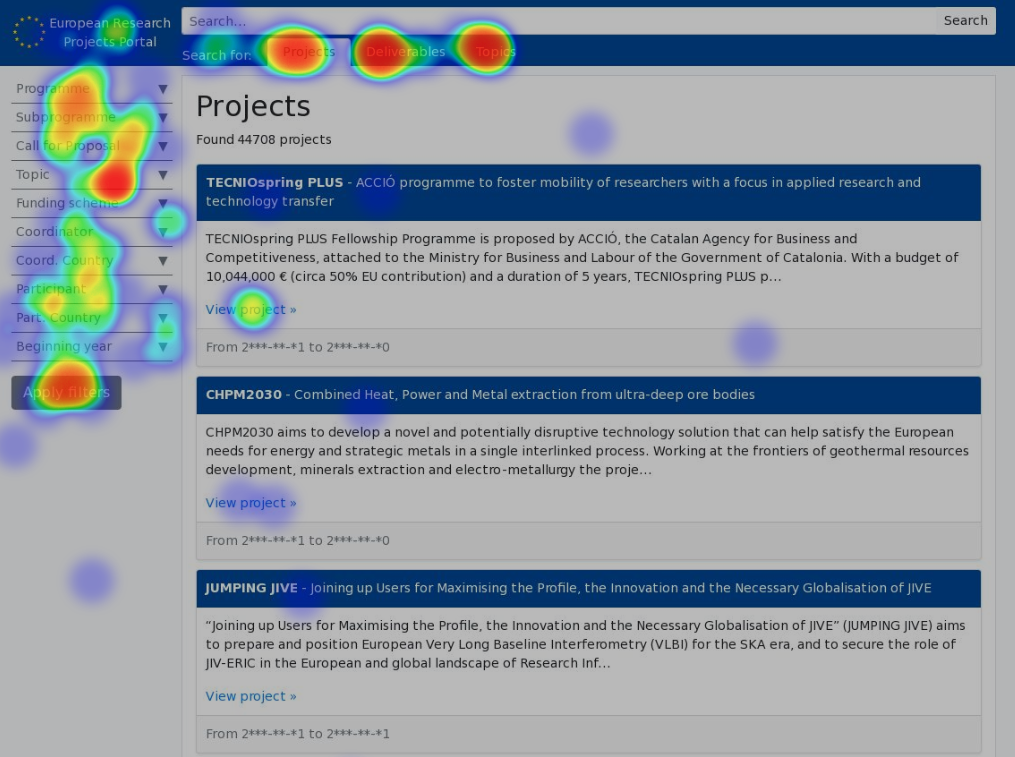
\includegraphics[width=\textwidth]{obrazky-figures/heatmap.png}
	\caption{Tepelná mapa klikání uživatelů na hlavní stránce portálu. Některé části obsahu stránky byly nástrojem pro sledování nahrazeny symbolem \uv{*} z důvodu možného výskytu citlivých údajů.}
	\label{img:heatmap}
\end{figure}

Výsledky tepelné mapy z obrázku~\ref{img:heatmap}, založené na statistice klikání uživatelů na hlavní stránce, jsou ovlivněny zaznamenáním interakce nejen s vyobrazenou stránkou, ale i částečně interakcí s modálním oknem, překrývajícím tento obsah. Z toho důvodu se v tepelné mapě vyskytují i zdánlivě neopodstatněné oblasti zájmu uživatelů.

Z mapy je patrné, že fasetová navigace je mezi uživateli velmi oblíbená. Uživatelé dále jeví zájem především o první zobrazený výsledek vyhledávání, část z nich si ale podrobněji prohlédne i výsledek umístěný na druhém místě.

Dále lze z mapy vyvodit i nedostatky uživatelského prostředí. Konkrétně ve výběru typu výsledků (\uv{Projects}, \uv{Deliverables}, \uv{Topics}) se uživatelé často snažili kliknout i na informativní popis \uv{Search for:}. Dalším poznatkem je nezájem uživatelů o vyhledávací pole. Napravení těchto nedostatků bude diskutováno v kapitole~\ref{section:improvements}.


\section{Rychlost obnovy dat}
Prázdnou databázi je možné naplnit 3483 dostupnými tématy výzev za TODO minut. Periodická obnova, prováděna jednou za TODO dní doplní v průměru TODO výzev a TODO jich aktualizuje. Tento proces trvá přibližně TODO minut.


\section{Možnost úprav}\label{section:improvements}
Současné řešení práce nabízí prostor pro další vylepšení. Za zmínku stojí například implementace našeptávače vyhledávacího vstupní pole pro jednodušší sepisování pokročilejších dotazů. Našeptávač by mohl uživateli nabízet jak názvy jednotlivých polí dokumentů, tak případně i hodnoty těchto polí. Přínosné by mohlo také být zvýraznění dvojice závorek nebo ověřování správnosti vstupu v reálném čase.

Vzhledem k automatickému plnění obsahu portálu může docházet k ukládání nepřesných informací. Pokud uživatel takovou informaci nalezne, bylo by vhodné dát mu možnost tuto situaci nahlásit. Tyto hlášení by mohly být vypsány v přehledu určeném pouze pro správce portálu, který by manuálně provedl nápravu. 

Dále by mohlo být užitečné přidat funkcionalitu \uv{hlídacího psa}, kdy by uživatel měl možnost zadat obory jeho zájmu a v případě otevření nové výzvy v daném oboru, by byl uživatel o této příležitosti bezprostředně informován.

V reakci na poznatky uvedené v kapitole~\ref{section:behaviour} lze upravit \blindtext



\chapter{Závěr}
Hlavním cílem této bakalářské práce bylo navrhnout a realizovat úpravu stávajícího portálu zaměřeného na výsledky evropských projektů. Portál byl úspěšně přetvořen s použitím novějších verzí technologií použitých v původním řešení a byly použity i technologie úplně nové. Do obsahu tohoto portálu byly úspěšně zakomponovány i témata výzev pro podávání návrhů nových projektů. Nad obsahem portálu lze provádět jak plnotextové tak i fasetové hledání. V případě potřeby je možné sestrojit pomocí dotazovacího jazyku sestrojit pokročilejší dotazy.

\blindtext % TODO zhodnocení

Řešení této práce mi bylo přínosné především rozšířením obzorů v~oblasti nerelačních databázi, hlubším pohledem do principů plnotextového vyhledáváním a také seznámením se s používáním systému Vue.js.